\documentclass[../main.tex]{subfiles}
\begin{document}

\ifSubfilesClassLoaded{\mainmatter}{}

\chapter{SeaQuest Experiment}
\label{ch:seaquest}

\section{Introduction}
SeaQuest is a fixed-target experiment utilizing the \SI{120}{\GeV} proton beam 
from the Fermilab Main Injector. Details of the SeaQuest spectrometer can be 
found in Ref.\ \cite{aidala2019}. A schematics of the spectrometer is shown in 
Fig.\ \ref{fig:spectrometer}. The target system consists of seven 
interchangeable targets, including a flask with liquid hydrogen, a flask with 
liquid deuterium,an empty flask (vacuum), solid carbon, iron, and tungsten 
targets as well as a space with no target (air). The targets are interchanged 
periodically to reduce systematic uncertainties in the measured cross section 
ratios for different targets.

The spectrometer consists of two magnets and four tracking stations. FMag, 
placed \SI{104}{\cm} downstream the target, is a \SI{5}{\m} solid iron magnet 
that acts as the beam dump as well as a focusing magnet. It is then followed by
the first tracking stations. Stations 1, 2 and 3 each consists of plastic 
scintillator hodoscopes and drift chambers. An open air dipole magnet (KMag) is
placed between station 1 and station 2. The vertical magnetic field from both 
magnets bends the muons horizontally, allowing the measurement of the momentum 
of the muons. Downstream of station 3, there is a 1 m iron wall acting as a 
hadron absorber. Station 4 is located behind the hadron absorber and acts as a 
muon identifier. Station 4 consists of a hodoscope array and 4 layers of 
proportional tube planes. Tracks that pass through the hadron absorber and 
produce hits on station 4 are assumed to be from muons. 
\pdfmargincomment{Should there be a dedicated section on the spectrometer?}

\begin{figure}[htbp!]
    \centering
    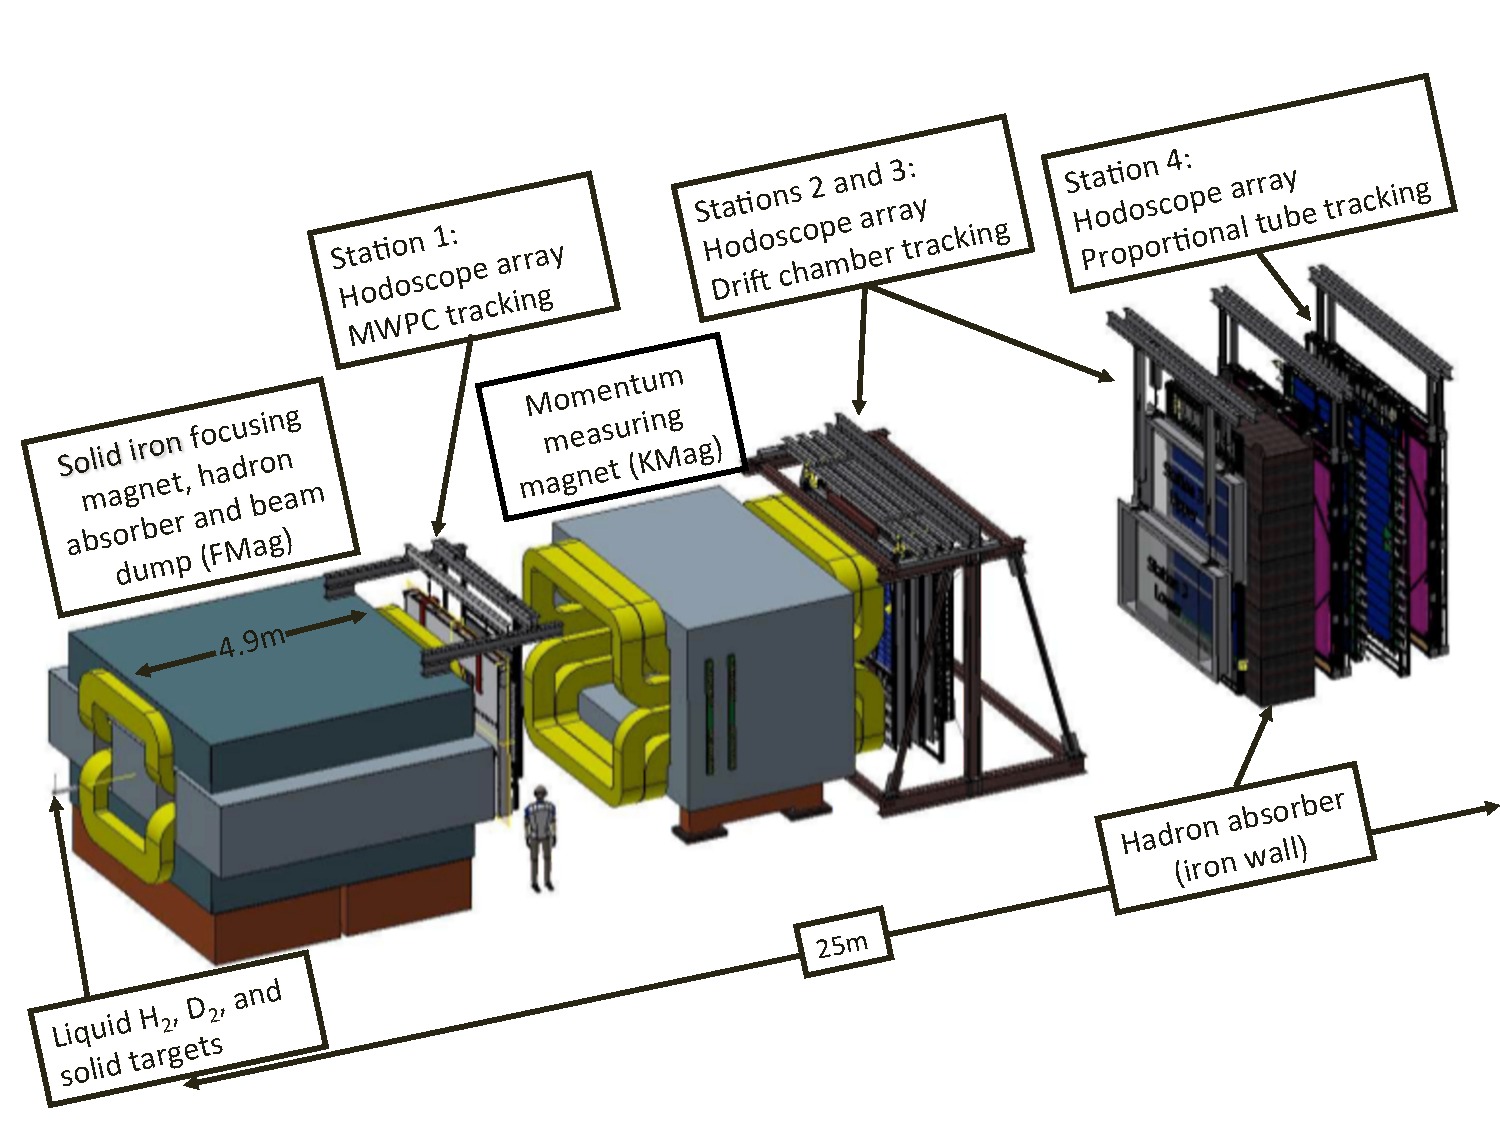
\includegraphics[width=0.6\linewidth]{SeaQuestSpectrometer}
    \caption{schematics of the SeaQuest spectrometer. Taken from Ref.\ 
		\cite{aidala2019}}
    \label{fig:spectrometer}
\end{figure}


\section{Beam}
\pdfmargincomment{A brief description of the beam structure, how the beam intensity 
	is monitor. And finally says that the varying instantaneous beam intensity 
	allows us to do intensity extrapolation which will be discussed in next 
	chapter}
The layout of the Fermilab accelerator complex is shown in Fig.\ \ref{fig:complex}.
SeaQuest received its \SI{120}{\GeV} proton beam from the Fermilab Main Injector.
The proton beam originate from a direct-extraction magnetron hydrogen ion source,
which produce a \SI{35}{\keV} negative hydrogen ion beam. It is then accelerated 
to \SI{750}{\keV} using Radio-frequency Quadrupole. Then the Linac accelrate the 
$H^-$ ions to \SI{400}{MeV}. The $H^-$ ions are then sent through a stripping foil 
to remove the electrons. The resulting proton beam then circulates in the Booster
accelerator and accelerates to \SI{8}{\GeV}. The \SI{8}{\GeV} proton beam is 
further accelerated by the Main Injector to \SI{120}{GeV}. The proton beam is 
extracted from the Main Injector using a process known as resonant extraction to 
provide a lower intensity beam over a 5 second spill. The extracted beam, which 
is sent to SeaQuest, retains the the \SI{53.1}{\MHz} structure of the Main 
Injector RF frequency, dividing hte beam in to ``RF buckets'' that are less than
\SI{2}{\ns} long and occur every \SI{18.8}{\ns}
\begin{figure}[htbp!]
	\centering
	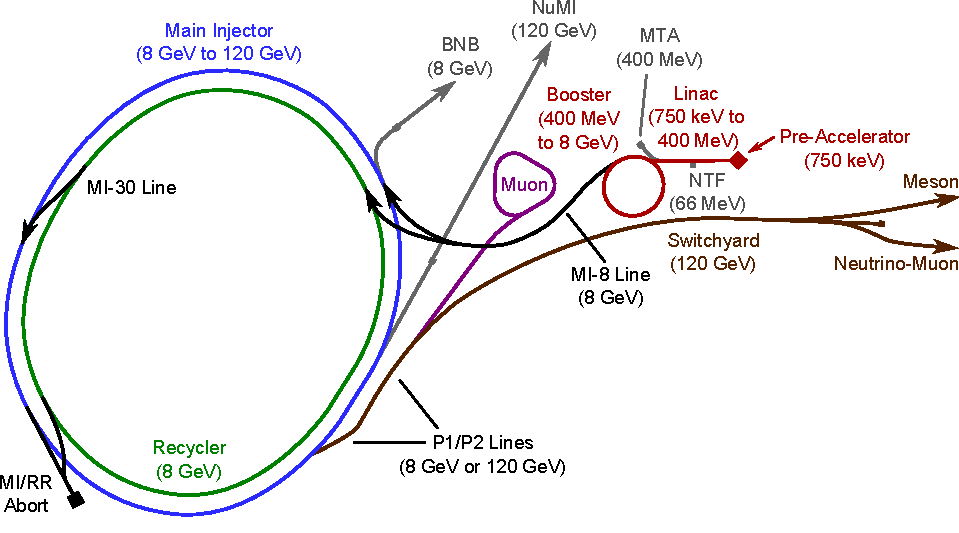
\includegraphics[width=0.6\linewidth]{Fermilab-complex}
	\caption{Layout of the Fermilab accelerator complex. Taken from Ref.\ \cite{concept-book}}
	\label{fig:complex}
\end{figure}
However the number of protons in each bucket varies greatly during the spill, as 
is shown in Fig.\ \ref{fig:intensity}.

The beam intensity is monitored using a Cerenkov counter, shown in Fig.\ \ref{fig:BIM}.
\begin{figure}[htbp!]
	\centering
	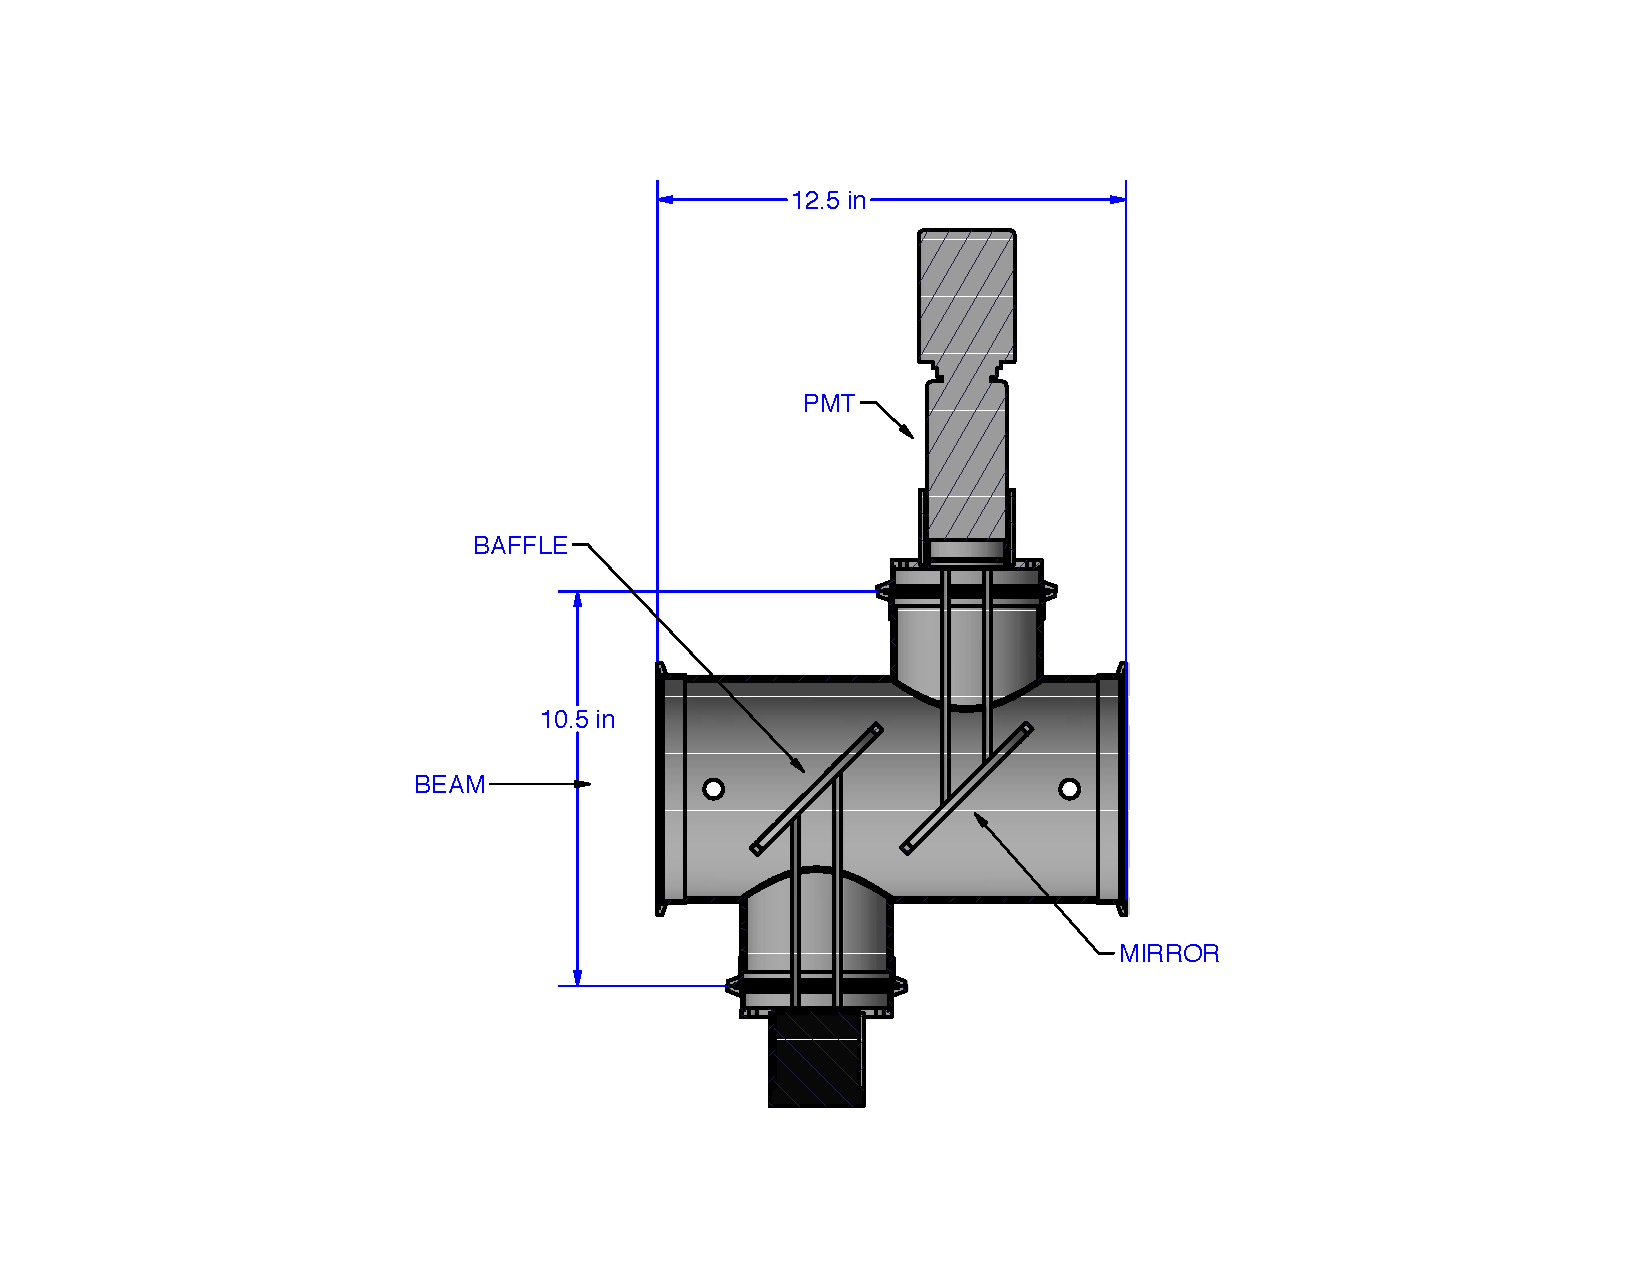
\includegraphics[width=0.6\linewidth]{BIMCerenkov}
	\caption{The Beam Intensity Monitor (BIM) Cerenkov counter. Taken from Ref.\
	\cite{aidala2019}.}
	\label{fig:BIM}
\end{figure}



\begin{figure}[htpb!]
	\centering
	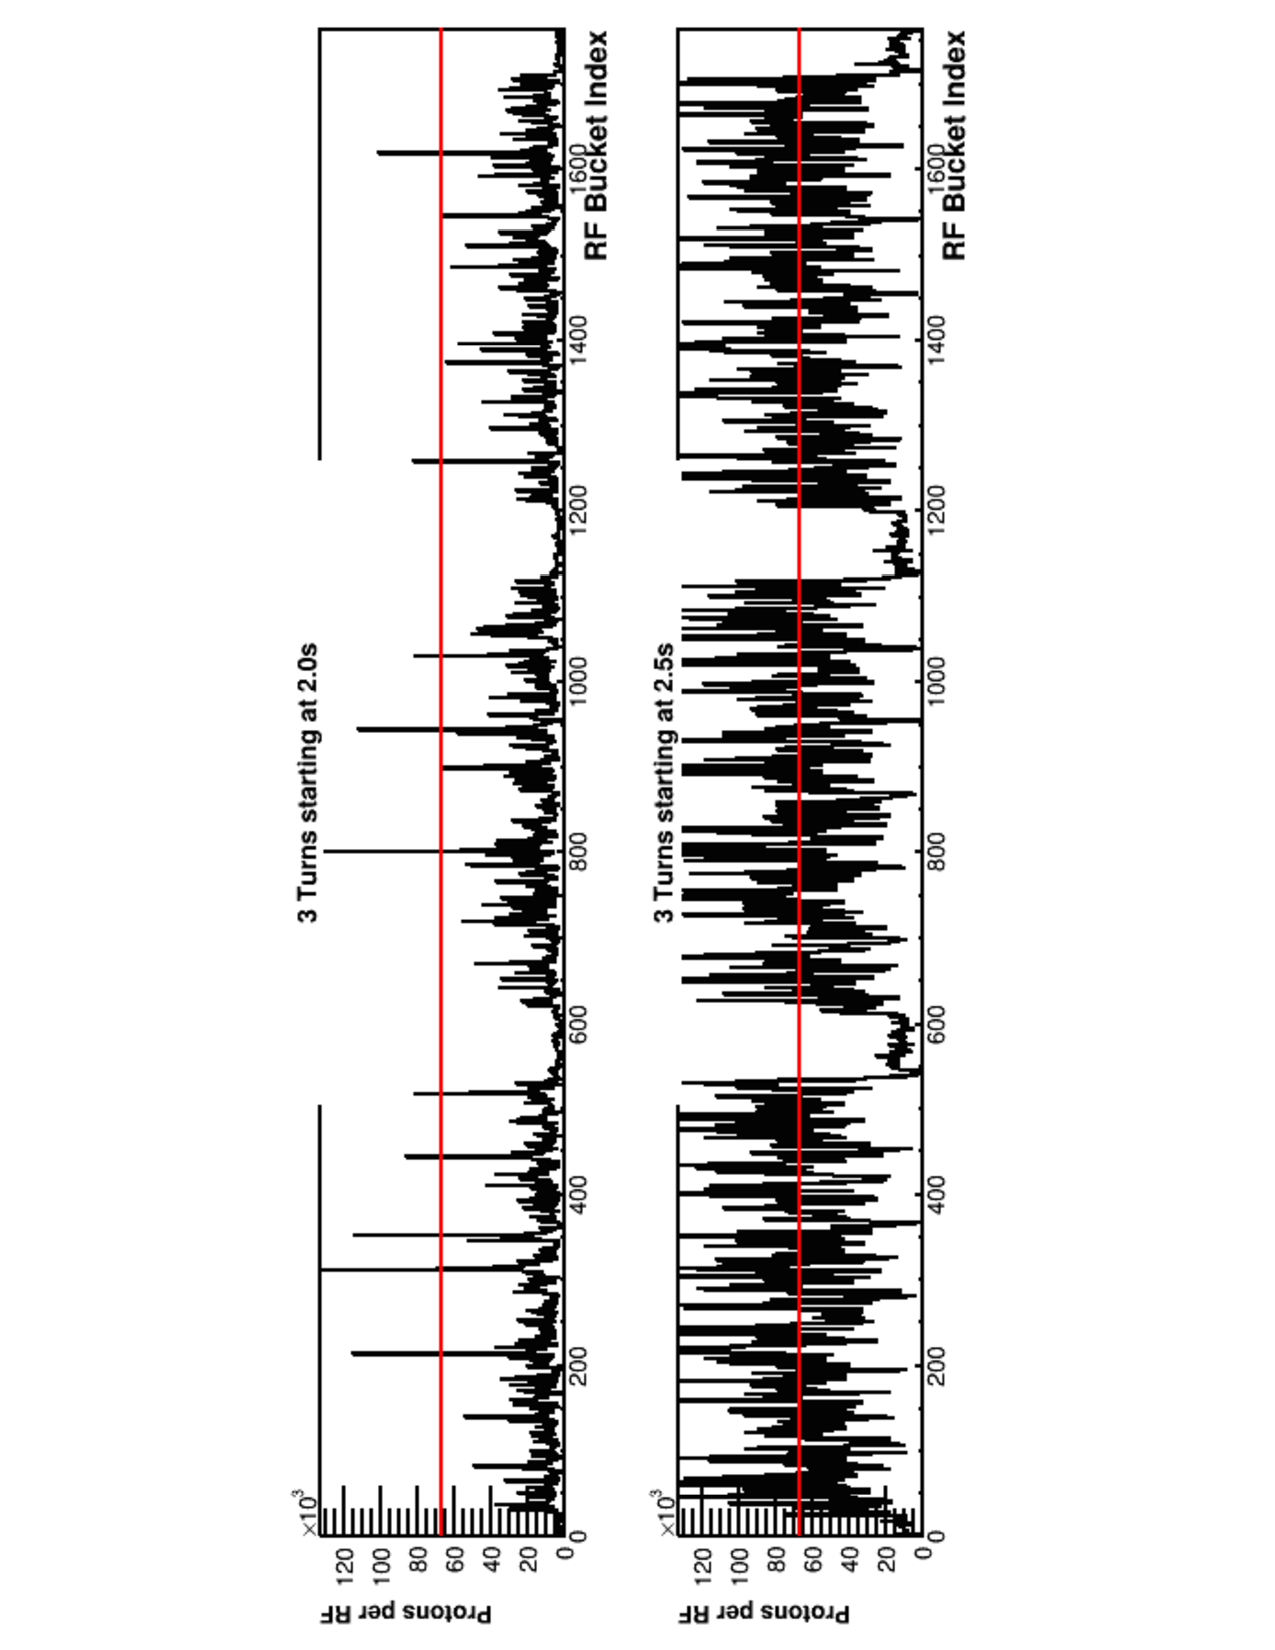
\includegraphics[width =0.8\linewidth, angle =270]{beam_intensity}
	\caption{The beam intensity measured by the Beam DAQ Cerenkov counter every 
		bucket. Taken from Ref.\ \cite{aidala2019}}
	\label{fig:intensity}
\end{figure}

\section{Target}
\pdfmargincomment{list the properties of the targets. Some past thesis quoted the
	wrong number. Check PDG}

\ifSubfilesClassLoaded{ \printbibliography[heading=bibintoc,title={References}]}{}
\end{document}
